\section{Примеры численного моделирования стабилизации неустойчивых решений}
\vspace{1em}

\subsection{Стабилизация неустойчивых решений}

\newtheorem{exmp_stbur}{Пример}

\begin{exmp_stbur}
\end{exmp_stbur}

Пусть $\theta_0 = \frac{sin(\pi x)}{G(x)}$ - начальное условие. Рассмотрим
стационарное решение уравнения Бюргерса с параметром $\tau$ возмем равный 15. 
В предыдущем параграфе показано неустойчивое поведение системы без управления. 
Cтабилизация указанного решения за счет управления с параметрами 
$\omega = (0, 0.4), \; r = 30, \; m = 4$ предоставлена ниже\\


\begin{figure}[H]
  \centering
  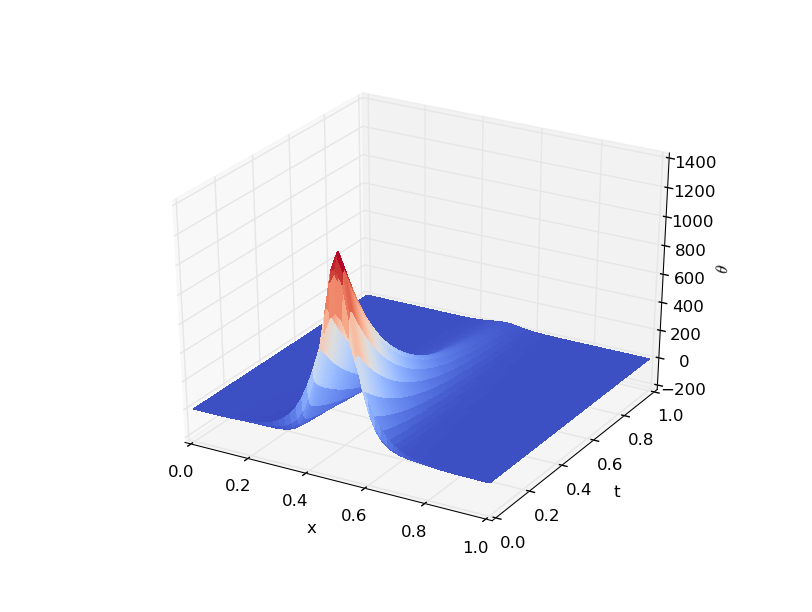
\includegraphics[width=4.0in]{re_s15}
  \caption{Управление с $\omega = (0, 0.4), \; m = 4, \; r = 30$}
  \label{fig:fig09}
\end{figure}


\begin{exmp_stbur}
\end{exmp_stbur}
Пусть теперь начальное условие системы $\theta_0(x) = \frac{x^2}{G(x)}$.
Вспомним, что чем больше параметр $\tau > 0$, тем сильнее он влияет на
неустойчивость нашей системы \eqref{fluct}. Зафиксируем следующие параметры
стабилизирующего оператора управления $\omega = (0, 0.4), \ r = 30$, а параметр 
$\tau$  возмем равный $15$. Неустойчивость этой системы продемонстирована в
предыдущем параграфе рис.~\ref{fig:fig08}. Ниже представлен процесс стабилизации

\begin{figure}[H]
 \centering
  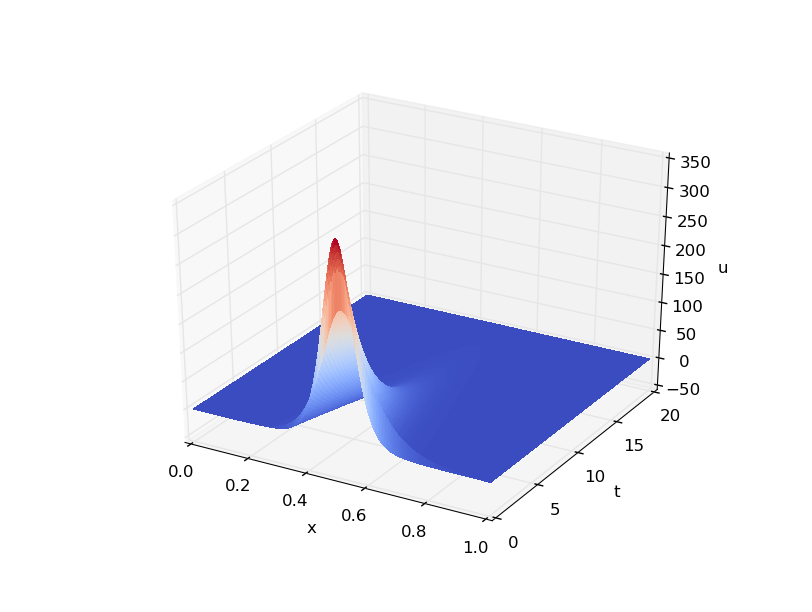
\includegraphics[width=4.0in]{re_x2_s15}
  \caption{Управление с $\omega = (0, 0.4), \; r = 30, \; m = 3$}
  \label{fig:fig10}
\end{figure}

\subsection{Анализ параметров оператора стабилизации}
\vspace{1em}

В данном параграфе проанализируем зависимости параметров стабилизации.

\begin{exmp_stbur}
\end{exmp_stbur}

Рассмотрим неустойчивое решение системы \eqref{linearized}, где $\tau = 11$,
$\theta_0 = \frac{sin(5 \pi x)}{G(x)}$. Зафиксируем параметры стабилизирующего
оператора $\omega = (0, 0.3)$, $m = 2$. Ниже представлена зависимость
поведения решения \eqref{linearized} от выбора параметра $r$.

\begin{figure}[H]
 \centering
  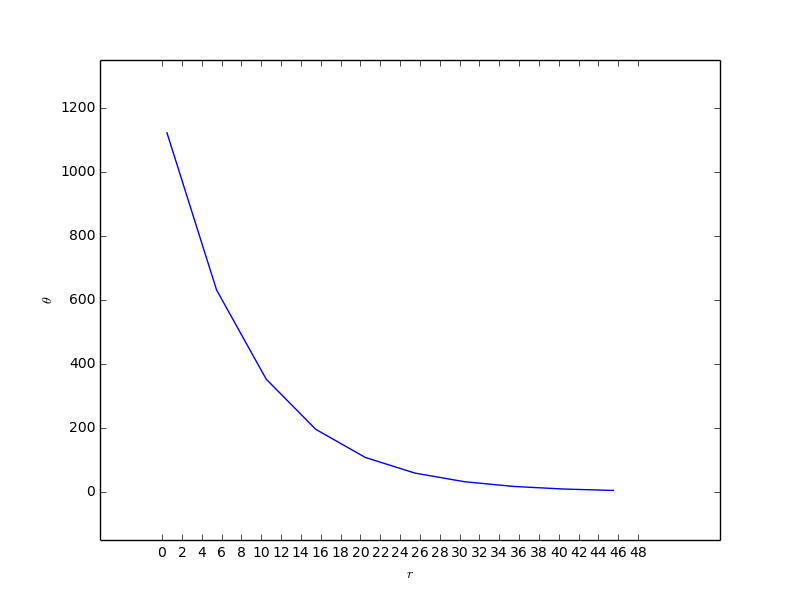
\includegraphics[width=4.0in]{r_m}
  \caption{$\omega = (0, 0.3), \; m = 2, \; r = 0.5, 5.5, ..., 45.5$}
  \label{fig:fig11}
\end{figure}

\begin{exmp_stbur}
\end{exmp_stbur}

Начальное условие и параметр $\tau$ семейства стационарных решений типа
shock-like оставим теми же, что и в предыдущем примере. На рис ~\ref{fig:fig12}
продемонстрирован график зависимости решения от выбора параметра $m$, при 
фиксированных $\omega = (0, 0.3)$ и $r = 50$.

\begin{figure}[H]
 \centering
  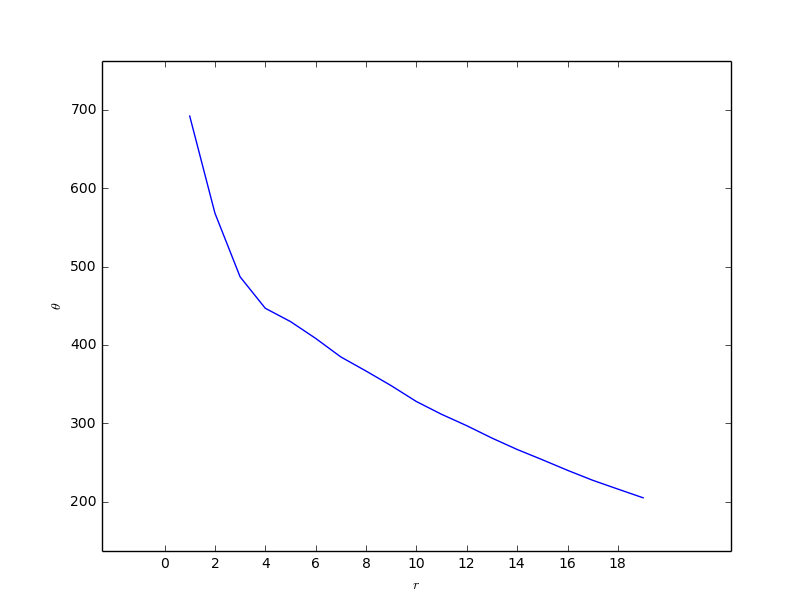
\includegraphics[width=4.0in]{m_r}
  \caption{$\omega = (0, 0.3), \; r = 50, \; m = 1, 2, .., 20$}
  \label{fig:fig12}
\end{figure}
